% Options for packages loaded elsewhere
\PassOptionsToPackage{unicode}{hyperref}
\PassOptionsToPackage{hyphens}{url}
\PassOptionsToPackage{dvipsnames,svgnames,x11names}{xcolor}
%
\documentclass[
  letterpaper,
  DIV=11,
  numbers=noendperiod]{scrartcl}

\usepackage{amsmath,amssymb}
\usepackage{iftex}
\ifPDFTeX
  \usepackage[T1]{fontenc}
  \usepackage[utf8]{inputenc}
  \usepackage{textcomp} % provide euro and other symbols
\else % if luatex or xetex
  \usepackage{unicode-math}
  \defaultfontfeatures{Scale=MatchLowercase}
  \defaultfontfeatures[\rmfamily]{Ligatures=TeX,Scale=1}
\fi
\usepackage{lmodern}
\ifPDFTeX\else  
    % xetex/luatex font selection
\fi
% Use upquote if available, for straight quotes in verbatim environments
\IfFileExists{upquote.sty}{\usepackage{upquote}}{}
\IfFileExists{microtype.sty}{% use microtype if available
  \usepackage[]{microtype}
  \UseMicrotypeSet[protrusion]{basicmath} % disable protrusion for tt fonts
}{}
\makeatletter
\@ifundefined{KOMAClassName}{% if non-KOMA class
  \IfFileExists{parskip.sty}{%
    \usepackage{parskip}
  }{% else
    \setlength{\parindent}{0pt}
    \setlength{\parskip}{6pt plus 2pt minus 1pt}}
}{% if KOMA class
  \KOMAoptions{parskip=half}}
\makeatother
\usepackage{xcolor}
\usepackage[top=30mm,left=20mm,heightrounded]{geometry}
\setlength{\emergencystretch}{3em} % prevent overfull lines
\setcounter{secnumdepth}{-\maxdimen} % remove section numbering
% Make \paragraph and \subparagraph free-standing
\makeatletter
\ifx\paragraph\undefined\else
  \let\oldparagraph\paragraph
  \renewcommand{\paragraph}{
    \@ifstar
      \xxxParagraphStar
      \xxxParagraphNoStar
  }
  \newcommand{\xxxParagraphStar}[1]{\oldparagraph*{#1}\mbox{}}
  \newcommand{\xxxParagraphNoStar}[1]{\oldparagraph{#1}\mbox{}}
\fi
\ifx\subparagraph\undefined\else
  \let\oldsubparagraph\subparagraph
  \renewcommand{\subparagraph}{
    \@ifstar
      \xxxSubParagraphStar
      \xxxSubParagraphNoStar
  }
  \newcommand{\xxxSubParagraphStar}[1]{\oldsubparagraph*{#1}\mbox{}}
  \newcommand{\xxxSubParagraphNoStar}[1]{\oldsubparagraph{#1}\mbox{}}
\fi
\makeatother


\providecommand{\tightlist}{%
  \setlength{\itemsep}{0pt}\setlength{\parskip}{0pt}}\usepackage{longtable,booktabs,array}
\usepackage{calc} % for calculating minipage widths
% Correct order of tables after \paragraph or \subparagraph
\usepackage{etoolbox}
\makeatletter
\patchcmd\longtable{\par}{\if@noskipsec\mbox{}\fi\par}{}{}
\makeatother
% Allow footnotes in longtable head/foot
\IfFileExists{footnotehyper.sty}{\usepackage{footnotehyper}}{\usepackage{footnote}}
\makesavenoteenv{longtable}
\usepackage{graphicx}
\makeatletter
\newsavebox\pandoc@box
\newcommand*\pandocbounded[1]{% scales image to fit in text height/width
  \sbox\pandoc@box{#1}%
  \Gscale@div\@tempa{\textheight}{\dimexpr\ht\pandoc@box+\dp\pandoc@box\relax}%
  \Gscale@div\@tempb{\linewidth}{\wd\pandoc@box}%
  \ifdim\@tempb\p@<\@tempa\p@\let\@tempa\@tempb\fi% select the smaller of both
  \ifdim\@tempa\p@<\p@\scalebox{\@tempa}{\usebox\pandoc@box}%
  \else\usebox{\pandoc@box}%
  \fi%
}
% Set default figure placement to htbp
\def\fps@figure{htbp}
\makeatother

\addtokomafont{disposition}{\rmfamily}
\KOMAoption{captions}{tableheading}
\usepackage{caption}
\usepackage{hyperref}
\usepackage[ocgcolorlinks]{ocgx2}
\usepackage{xcolor}
\hypersetup{colorlinks,linkcolor={blue},citecolor={purple}, colorlinks=true, citecolor={blue}, urlcolor={blue}}
\makeatletter
\@ifpackageloaded{caption}{}{\usepackage{caption}}
\AtBeginDocument{%
\ifdefined\contentsname
  \renewcommand*\contentsname{Table of contents}
\else
  \newcommand\contentsname{Table of contents}
\fi
\ifdefined\listfigurename
  \renewcommand*\listfigurename{List of Figures}
\else
  \newcommand\listfigurename{List of Figures}
\fi
\ifdefined\listtablename
  \renewcommand*\listtablename{List of Tables}
\else
  \newcommand\listtablename{List of Tables}
\fi
\ifdefined\figurename
  \renewcommand*\figurename{Figure}
\else
  \newcommand\figurename{Figure}
\fi
\ifdefined\tablename
  \renewcommand*\tablename{Table}
\else
  \newcommand\tablename{Table}
\fi
}
\@ifpackageloaded{float}{}{\usepackage{float}}
\floatstyle{ruled}
\@ifundefined{c@chapter}{\newfloat{codelisting}{h}{lop}}{\newfloat{codelisting}{h}{lop}[chapter]}
\floatname{codelisting}{Listing}
\newcommand*\listoflistings{\listof{codelisting}{List of Listings}}
\makeatother
\makeatletter
\makeatother
\makeatletter
\@ifpackageloaded{caption}{}{\usepackage{caption}}
\@ifpackageloaded{subcaption}{}{\usepackage{subcaption}}
\makeatother

\usepackage[round]{natbib}
\bibliographystyle{apalike}
\usepackage{bookmark}

\IfFileExists{xurl.sty}{\usepackage{xurl}}{} % add URL line breaks if available
\urlstyle{same} % disable monospaced font for URLs
\hypersetup{
  pdftitle={Indicator 5.3.3: Political Party Engagement with Health and Climate Change},
  pdfauthor={Zachary P. Dickson \& Cornelius Erfort},
  colorlinks=true,
  linkcolor={blue},
  filecolor={Maroon},
  citecolor={Blue},
  urlcolor={Blue},
  pdfcreator={LaTeX via pandoc}}


\title{Indicator 5.3.3: Political Party Engagement with Health and
Climate Change}
\author{Zachary P. Dickson \& Cornelius Erfort}
\date{2025-04-08}

\begin{document}
\maketitle


\section{Indicator 5.3.1: Political party engagement with health and
climate
change}\label{indicator-5.3.1-political-party-engagement-with-health-and-climate-change}

\textbf{Main Text:}

A key obstacle to consolidating political commitment to address the
climate crisis remains electing politicians and parties who prioritise
climate change and its associated risks to public health. This indicator
tracks European political parties' emphasis of public health and climate
change in official party communication via press releases. The indicator
is based on over 550,000 press releases from 139 political parties in 23
EU countries and the UK, covering a period from 2010 to 2025. The data
were analysed using a fine-tuned language model trained validated to
identify the primary substantive focus of the press releases. The
results are presented according to the associated party family of each
party. The figure highlights the dramatic influence that the COVID-19
pandemic had on the political agenda, with a significant increase in
press releases addressing public health in 2020 and 2021. However, the
data also show that press releases focusing on climate change has
remained relatively stable over the past 15 years, with Green parties a
notable exception. Green, Liberal and Conservative parties are the most
likely to link public health to climate change, while radical right-wing
parties are the least likely to do so. At the height of the pandemic in
2020, nearly 250 press releases were issued by social democratic parties
that framed climate change as a public health issue. Yet, these numbers
have since declined, with parties focusing on the climate-health nexus
in only about one percent of their press releases in 2024.

\pandocbounded{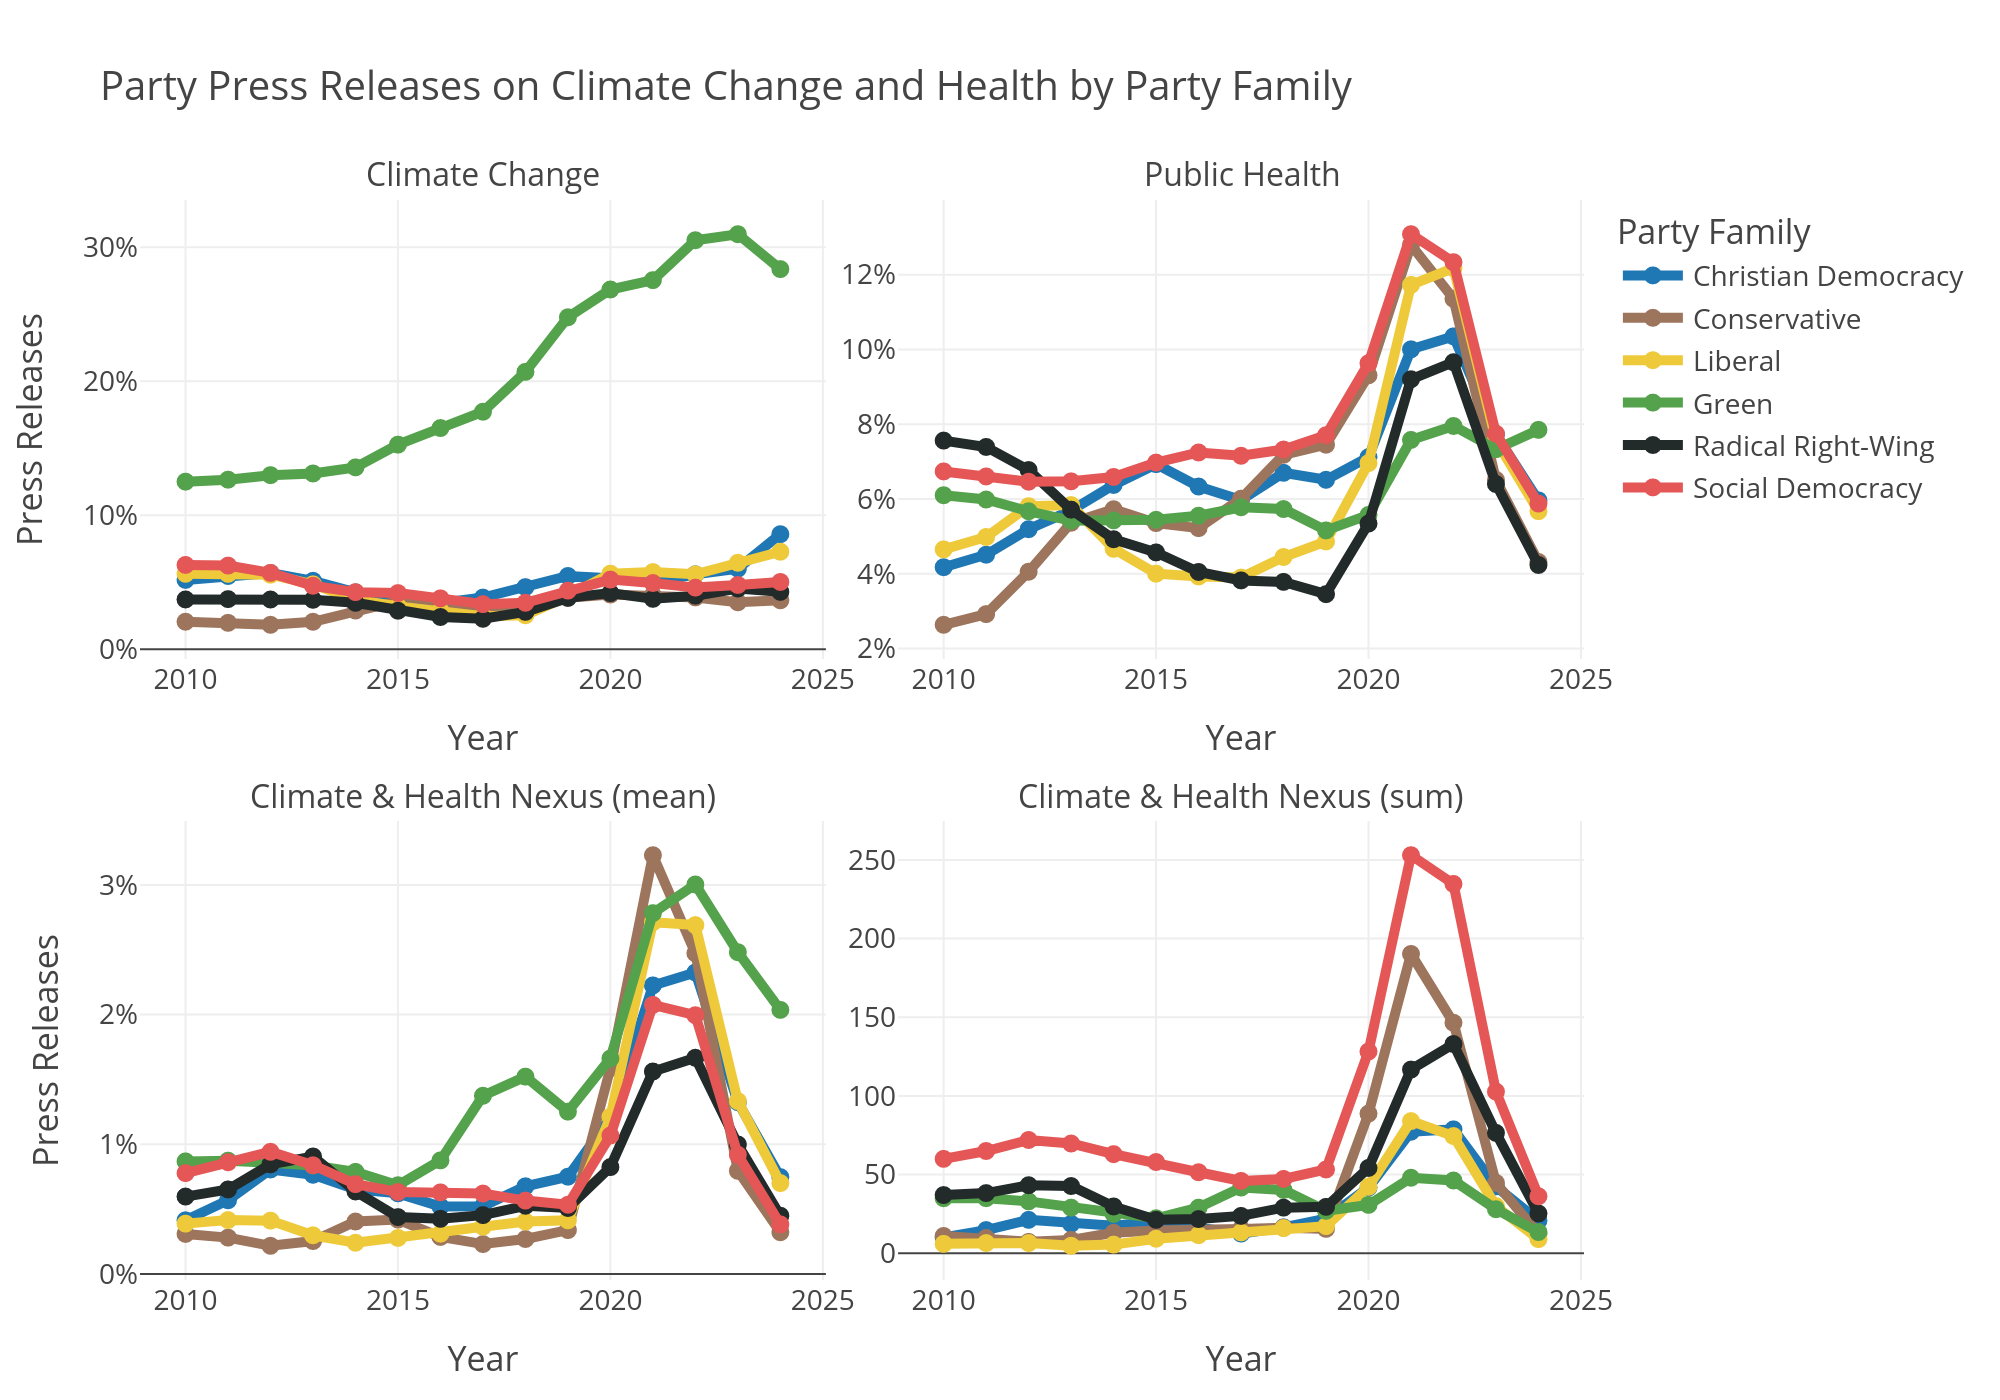
\includegraphics[keepaspectratio]{indicator_5_3_3.png}}

\newpage

\section{Appendix}\label{appendix}

\subsection{Indicator 5.3.3}\label{indicator-5.3.3}

\subsubsection{Political party engagement with health and climate
change}\label{political-party-engagement-with-health-and-climate-change}

This indicator tracks European political parties' emphasis of public
health and climate change in official party communication via press
releases. The indicator is based on over 550,000 press releases from 139
political parties in 23 EU countries and the UK, covering a period from
2010 to 2025. The data were analysed using a validated fine-tuned
language model trained on pre-labeled data that identifies the primary
substantive focus of the press releases. The results are presented
according to the party family according to ParlGov. The figure
highlights the dramatic influence that the COVID-19 pandemic had on the
political agenda, with a significant increase in press releases
addressing public health in 2020 and 2021. However, the data also show
that press releases focusing on climate change has remained relatively
stable over the past 15 years, with Green parties a notable exception.
Social Democratic, Liberal and Conservative parties are the most likely
to link public health to climate change, while radical right-wing
parties are the least likely to do so. At the height of the pandemic in
2020, nearly 250 press releases were issued by social democratic parties
that framed climate change as a public health issue. However, these
numbers have since declined, with parties focusing on the climate-health
nexus in only about one percent of their press releases in 2024.

\subsubsection{Geographic coverage of
Europe}\label{geographic-coverage-of-europe}

This indicator covers 23 EU countries and the UK. The countries included
are: Poland, Germany, Ireland, Netherlands, Slovenia, Denmark, Hungary,
Austria, Sweden, Bulgaria, Spain, Croatia, Finland, United Kingdom,
Greece, Switzerland, Estonia, France, Portugal, Cyprus, Slovakia, Italy,
Czech Republic, and Belgium. The countries were selected based on the
availability of press releases from political parties.

\subsubsection{Methods}\label{methods}

The data were analysed using a fine-tuned language model trained on
pre-labeled data that identifies the primary substantive focus of the
press releases. The model is trained to predict the substantive focus of
the press releases based on the text of the press release. The
classification scheme is based on the Comparative Agendas Project (CAP)
\citep{walgrave2019comparative} which includes the following categories:
defense, technology, culture, macroeconomics, domestic commerce,
immigration, healthcare, government operations, housing, social welfare,
education, agriculture, environment and climate, foreign trade, civil
rights, energy, international affairs, labor, law and crime,
transportation, and public lands. One small modification was made to
change the focus of the category ``environment'' to ``environment and
climate'' to better reflect the focus of the indicator.

The model was trained on a dataset of over 15,000 press releases that
were randomly sampled from various political parties across Europe
(e.g.~the entire dataset). The training dataset was labelled using
OpenAI's GPT-4 model \citep{achiam2023gpt}, which was used as a
zero-shot classifier to predict the substantive focus of the press
releases according to the modified CAP classification scheme. The
training dataset was then manually reviewed and corrected by a team of
researchers to ensure the accuracy of the labels. A multilingual
xlm-RoBERTA-L model trained by Facebook AI \citep{xlm_roberta} was used
as the base model for the fine-tuning process. The model achieved a
weighted F1 score of 0.86 on the training dataset, indicating a high
level of accuracy in predicting the substantive focus of the press
releases. Full results of the model evaluation are presented below. The
model has been made publicly available on HuggingFace at:
\url{https://huggingface.co/z-dickson/xlm-roberta-large-political-issues}.

\begin{table}[ht]
\caption{Classification Report for Fine-tuned xlm-RoBERTA-L Model}
\centering
\begin{tabular}{lcccc}
\hline
\textbf{Class} & \textbf{Precision} & \textbf{Recall} & \textbf{F1-Score} & \textbf{Support} \\
\hline
0  & 0.88 & 0.89 & 0.89 & 307 \\
1  & 0.86 & 0.88 & 0.87 & 76 \\
2  & 0.93 & 0.96 & 0.95 & 162 \\
3  & 0.99 & 0.91 & 0.95 & 97 \\
4  & 0.83 & 0.83 & 0.83 & 139 \\
5  & 0.89 & 0.91 & 0.90 & 147 \\
6  & 0.94 & 0.89 & 0.92 & 180 \\
7  & 0.77 & 0.91 & 0.83 & 44 \\
8  & 0.89 & 0.81 & 0.84 & 98 \\
9  & 0.82 & 0.92 & 0.87 & 74 \\
10 & 0.86 & 0.89 & 0.88 & 79 \\
11 & 0.75 & 0.70 & 0.72 & 43 \\
12 & 0.91 & 0.83 & 0.87 & 48 \\
13 & 0.40 & 0.33 & 0.36 & 6 \\
14 & 0.69 & 0.92 & 0.79 & 66 \\
15 & 0.57 & 1.00 & 0.73 & 4 \\
16 & 0.89 & 0.67 & 0.76 & 24 \\
17 & 0.84 & 0.89 & 0.87 & 180 \\
18 & 0.69 & 0.45 & 0.55 & 91 \\
19 & 0.00 & 0.00 & 0.00 & 1 \\
20 & 0.81 & 1.00 & 0.89 & 17 \\
\hline
\textbf{Accuracy}     &       &       & \textbf{0.86} & 1883 \\
\textbf{Macro Avg}    & 0.77  & 0.79  & 0.77  & 1883 \\
\textbf{Weighted Avg} & 0.86  & 0.86  & 0.86  & 1883 \\
\hline
\end{tabular}

\end{table}

After the model was trained and evaluated, it was used to classify each
of the press releases in the dataset. These classifications were then
used to create a time series of focus on public health and climate
change in the press releases. The time series was created by aggregating
the annual number of press releases devoted to climate change, public
health, and the intersection between climate change and public health.
The time series was then visualized using a line graph, with the x-axis
representing the year and the y-axis representing the number of press
releases in each category. The results are presented according to the
party family according to ParlGov \citep{doring2012parliament}.

\subsubsection{Data sources}\label{data-sources}

All data were collected from the official websites of the political
parties and included press releases from 2010 to 2025. Data collected
for the indicator builds upon previous work in
\citet{erfort2023partypress} and \citet{dickson2024going}. Data were
collected using a web scraping tool that automatically downloaded the
press releases from the official websites of the political parties. The
data were then cleaned and pre-processed to remove any irrelevant
information, such as HTML tags and formatting. The final dataset
included 553,675 press releases from 139 political parties in 23 EU
countries and the UK.

\subsubsection{Caveats/Limitations}\label{caveatslimitations}

The indicator is based on press releases from political parties, which
may not accurately reflect the full range of political discourse on
health and climate change. The data are also limited to the countries
included in the analysis, which may not be representative of the entire
European Union. Additionally, the model used to classify the press
releases is not perfect and may misclassify some press releases. The
model was trained on a dataset of over 15,000 press releases, but it is
possible that some press releases were misclassified due to the
complexity of the language used in the press releases. Finally, there
are differences in the ways in which political parties utilize press
releases, which may affect the results. For example, some parties may
issue more press releases than others, or may use different language to
describe similar issues. This may lead to differences in the number of
press releases issued by different parties, which may affect the results
of the analysis.

\subsubsection{Future form of the
indicator}\label{future-form-of-the-indicator}

The indicator will be updated annually to include new data and to
reflect changes in the political landscape. The model used to classify
the press releases will also be updated periodically to improve its
accuracy and to reflect changes in the language used in the press
releases. The indicator will also be expanded to include additional
countries and political parties, as well as additional data sources,
such as social media and news articles. This will allow for a more
comprehensive analysis of the political discourse on health and climate
change in Europe.

The indicator will also be expanded to include additional data sources,
such as manifestos and parliamentary speeches. This will allow for a
more comprehensive analysis of the political discourse on health and
climate change in Europe. The indicator will also be expanded to include
additional countries and political parties, as they become available.
This will allow for a more comprehensive analysis of the political
discourse on health and climate change in Europe.

\subsubsection{Additional analysis}\label{additional-analysis}

The indicator will also be expanded to include additional analyses that
capture party positions on health and climate change. These future
analyses will be used to assess the party's positions on health and
climate change, as well as the party's overall engagement with these
issues. The results of these analyses will be presented in future
reports and will be used to inform policy recommendations for improving
political engagement with health and climate change in Europe.

\newpage


\renewcommand\refname{References}
  \bibliography{references.bib}



\end{document}
